\RequirePackage{times}
\RequirePackage[scaled=0.92]{helvet}
\documentclass[article,11pt,oneside]{memoir}
\usepackage{amsmath}
\usepackage{mtpro2}
\usepackage[squaren]{SIunits}
\usepackage{booktabs}
\usepackage{graphicx}
\usepackage[abbreviate=true,biblabel=brackets,biochem=false,maxauthors=15,super=true,usetitle=true]{achemso}

\bibliographystyle{achemso}
\graphicspath{{images/}}

\usepackage{lastpage}
\makepagestyle{eli}
\makeoddhead{eli}{2009 Creatinine Reverificiation}{}{\thepage\ of \pageref{LastPage}}
\pagestyle{eli}

\title{Syva Creatinine Validity Test: Periodic Reverification on The Hitachi 717 Chemistry Analyzer}
\author{ElSohly Laboratories}
\date{\today}

\setlength{\droptitle}{-3em}
\pretitle{\noindent\Large\bfseries} 
\posttitle{\vskip 1em\par\vskip 1em}
\preauthor{\noindent\large\lineskip 0.5em}%
%\begin{tabular}[t]{l}}
%\postauthor{\end{tabular}\par\vskip 1em}
\postauthor{\vskip 1em\par\vskip 1em}
\predate{\noindent\large}
\postdate{\par} 

\settypeblocksize{9.0in}{6.5in}{*}
\setulmargins{1.0in}{*}{*}
\setlrmargins{*}{1in}{*}
%\setheadfoot{14pt}{14pt}
\checkandfixthelayout

\begin{document}
\maketitle
\tableofcontents
\chapter{Purpose}
An annual reverification of the Syva Creatinine Validity Test is performed to establish that the analytical methodology remains valid.

\chapter{Instrumentation and Parameters}
A Hitachi 717 running System FD version 7176000-04-07 with Data FD version 7176001-00-01 was used to analyze study samples.
Data processing and calculations were performed with the R software environment version 2.8.1\cite{R-Development-Core-Team:2008th} using results produced by the instument.
The instrument was set to use the following parameters:

\begin{minipage}{3in}
\begin{verbatim}
CHEMISTRY PARAMETERS

TEST              [CR   ]
ASSAY CODE        [RATE-A  ]:[28]-[31]
SAMPLE VOLUME     [ 8][ 8]
R1 VOLUME         [250][100][NO ]
R2 VOLUME         [50 ][ 50][NO ]
WAVELENGTH        [570][505]
CALIB. METHOD     [LINEAR   ][0][0]
STD.(1) CONC.-POS.[  0.0]-[16]
STD.(2) CONC.-POS.[  2.0]-[17]
STD.(3) CONC.-POS.[     ]-[ 0]
STD.(4) CONC.-POS.[     ]-[ 0]
STD.(5) CONC.-POS.[     ]-[ 0]
STD.(6) CONC.-POS.[     ]-[ 0]
SD LIMIT          [  999]
DUPLICATE LIMIT   [32000]
SENSITIVITY LIMIT [    0]
ABS.LIMIT(INC/DEC)[32000][INCREASE]
PROZONE LIMIT     [     0][UPPER]
EXPECTED VALUE    [  20.0]-[ 400.0]
TECH. LIMIT       [  -0.1]-[ 400.0]
INSTRUMENT FACTOR [ 1.0]
\end{verbatim}
\end{minipage}

\chapter{LOD/ULOL}
\section{Description of Methods}
The limit of quantitation (LOQ) and limit of linearity (ULOL) are reverified at the 0.5 and \unit{300}{\milli\gram\per\deci\liter} levels, respectively.
Quintuple analyses are performed at each point, and the resulting data are used to calculate the mean and sample standard deviation.
The criteria for reverification are results within \(\pm 20\%\) of the target values.

\section{Summary of Statistical Data}
\begin{center}
\begin{tabular}{lr@{.}lr@{.}l}
\toprule
 & \multicolumn{4}{c}{\em Control point} \tabularnewline \cmidrule(l){2-5}
 & \multicolumn{2}{c}{\unit{0.5}{\milli\gram\per\deci\liter}} &  \multicolumn{2}{c}{\unit{300.0}{\milli\gram\per\deci\liter}} \tabularnewline \midrule
Mean & 0 & 5 & 256 & 9 \tabularnewline
SD & 0 & 04 & 4 & 09 \tabularnewline
CV\% & 9 & 3 & 1 & 6 \tabularnewline
\bottomrule
\end{tabular}
\end{center}

\section{Discussion}
All results were within \(\pm 20\%\) of the target values.

\chapter{Carryover}
The extent of carryover from samples at extreme out-of-range concentrations (X) of 0 and \unit{1000}{\milli\gram\per\deci\liter} to samples at the \unit{2}{\milli\gram\per\deci\liter} (D) decision point is evaluated annually.

\section{Description of Methods}
Carryover studies are performed using the method of \citeauthor{Armbruster:1993pb}\cite{Armbruster:1993pb} with the sequence
\[
\mathrm{D_1\,D_2\,D_3\,X_1\,X_2\,D_4\,X_3\,X_4\,D_5\,D_6\,D_7\,D_8\,X_5\,X_6\,D_9\,X_7\,X_8\,D_{10}\,X_9\,X_{10}\,D_{11}.}
\]
Percent carryover is evaluated as the percent difference in response of carryover candidate samples vs normal samples
\[
100\times\frac{\LEFTRIGHT[]{\mathrm{D_4 + D_5 + D_9 + D_{10} + D_{11}}} - \LEFTRIGHT[]{\mathrm{D_2 + D_3 + D_6 + D_7 + D_8}}}{\LEFTRIGHT[]{\mathrm{D_2+ D_3 + D_6 + D_7 + D_8}}}.
\]
Two-sample {\em t} tests using pooled variances are used to compare the means between carryover candidates and the decision point, 
\begin{equation*}
\LEFTRIGHT.\rcbrace{
\begin{aligned}
H_0\!: & & \mu_{\mathrm D} - \mu_{\mathrm X} &= 0.4, \\
H_a\!: & & \mu_{\mathrm D} - \mu_{\mathrm X} &< 0.4,
\end{aligned}
}
\qquad \text{for blank carryover} 
\end{equation*}
\begin{equation*}
\LEFTRIGHT.\rcbrace{
\begin{aligned}
H_0\!: & &\mu_{\mathrm X} - \mu_{\mathrm D} &= 0.4, \\ 
H_a\!: & &\mu_{\mathrm X} - \mu_{\mathrm D} &< 0.4,
\end{aligned}
}
\qquad \text{for \unit{1000}{\milli\gram\per\deci\liter} carryover.}
\end{equation*}
The \unit{0.4}{\milli\gram\per\deci\liter} level is chosen for comparison as it  constitutes 20\% of the decision point value.
Carryover is expected to bias results in the direction of the carryover concentration and the result is evaluated at a significance level \(\alpha = 0.01.\) 

\section{Analytical Results}
\begin{center}
\begin{tabular}{lr@{.}lr@{.}l}
\toprule
 & \multicolumn{4}{c}{\em Carryover level} \tabularnewline \cmidrule(l){2-5}
 & \multicolumn{2}{l}{\unit{0}{\milli\gram\per\deci\liter}} &  \multicolumn{2}{l}{\unit{1000}{\milli\gram\per\deci\liter}} \tabularnewline \midrule
Carryover \% & 2 & 0 & -3 & 0 \tabularnewline                                            
{\em p-}value  & 4 & \(7\times 10^{-8}\) & 3 & \(3\times 10^{-8}\) \tabularnewline
\bottomrule
\end{tabular}
\end{center}

\section{Discussion}
Carryover from blank and \unit{1000}{\milli\gram\per\deci\liter} samples was determined to be a relatively insignificant factor.
In both cases, the {\em t} tests support (i.e., \(p\le \alpha\)) the conclusion that the difference in means between carryover candidates and decision point samples is less than 20\% of the decision point cutoff.
In addition, the apparent carryover followed a gradient opposite to the hypothetical bias that would be expected.

\chapter{Specificity/Interference}
Specificity studies are performed to assess the ability of the assay to discriminate the following substances from creatinine at the levels indicated:
\begin{center}
  \begin{tabular}{ll}
    \toprule
    Ascorbic acid & 20, 50, and \unit{100}{\milli\gram\per\milli\liter} \tabularnewline
    Niacin  & 3.0, 7.5, and \unit{15.0}{\milli\gram\per\milli\liter} \tabularnewline
    Tropicana Apple Juice with Vitamin C  & undiluted \tabularnewline
    Mountain Dew  & undiluted \tabularnewline
    Visine Original & undiluted \tabularnewline
    \bottomrule
  \end{tabular}
\end{center}

\section{Description of Methods}
Units of concentration are converted to milligrams per deciliter for statistical calculations.
Linear regression of the response, \(R,\) on concentration, \(C,\)
\[
\mathrm{E}(R/C) = \beta_0 + \beta_1 C,
\]
is performed for analytes that are tested at multiple concentrations.
Percent cross-reactivity is calculated as
\[
100 \times \frac{C_d}{C_a} = 100 \times \frac{20.0\beta_1}{20.0 - \beta_0},
\]
where \(C_d/C_a\) is the ratio of the creatinine decision-point cutoff concentration, \(C_d,\) to the concentration of interfering analyte that is necessary to elicit an equivalent response, \(C_a\).

\section{Analytical Results}
Undiluted Visine Original, Tropicana Apple Juice, and Mountain Dew produce responses of 0.1, 4.9, and \unit{20.4}{\milli\gram\per\deci\liter}, respectively.
See Figure \ref{ascorbate} for a graphical summary of the cross-reactivity data of the vitamins.
\begin{center}
\begin{tabular}{lr@{.}lr@{.}lr@{.}l}
\toprule
 & \multicolumn{4}{c}{\em Linear Regression Coefficients} & \multicolumn{2}{l}{} \tabularnewline\cmidrule(lr){2-5}
{\em Analyte} & \multicolumn{2}{l}{\(\beta_0\)} & \multicolumn{2}{l}{\(\beta_1\)} & \multicolumn{2}{l}{{\em Cross-reactivity, \%}} \tabularnewline\midrule
Ascorbic acid & 1 & 80 & 2 & \(44\times 10^{-3}\) & 0 & 3 \tabularnewline
Niacin & -0 & 02 & 1 & \(08\times 10^{-3}\) & 0 & 1 \tabularnewline
\bottomrule
\end{tabular}
\end{center}

\begin{figure}[h!]
\centering
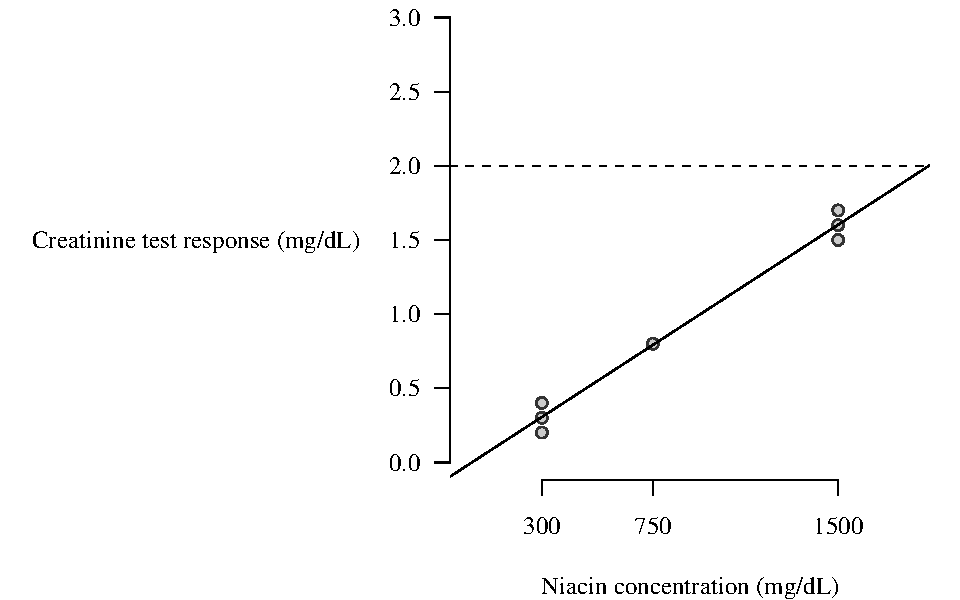
\includegraphics[scale=0.63]{b3}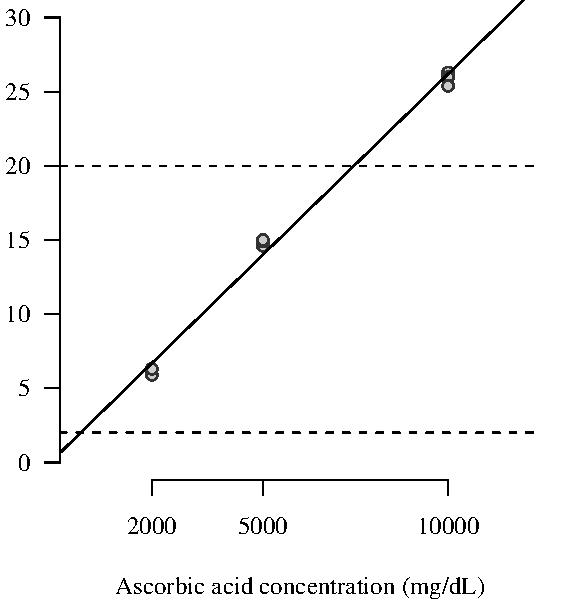
\includegraphics[scale=0.63]{aa}
\caption{Cross-reactivities of niacin and ascorbic acid. Decision points are indicated by dashed lines.}
\label{ascorbate}
\end{figure}

\section{Discussion}
Both ascorbic acid and niacin possess a vanishingly small percentage of cross-reactivity at the \unit{20}{\milli\gram\per\deci\liter} decision point.
Visine Original, Tropicana Apple Juice, and Mountain Dew produce responses below, between, and above both decision points, respectively.

\chapter{Conclusions}
\begin{enumerate}
\item The LOQ and ULOL were reverified at the 0.5 and \unit{300}{\milli\gram\per\deci\liter} levels, respectively.
\item No evidence for carryover was found for candidate samples at the \unit{2.0}{\milli\gram\per\deci\liter} decision point following blank or \unit{1000}{\milli\gram\per\deci\liter} samples.
\item The cross-reactivities of the vitamins ascorbic acid and niacin, and the assay response to several commercially available products with superficial similarity to urine was characterized.
\end{enumerate}
This method meets requirements for reverification, and is valid for analysis of forensic urine samples under the Federal guidelines for a drug-free workplace.

\bibliography{validation}

\end{document}
